\documentclass[twoside,english]{uiofysmaster}
%\bibliography{references}

\usepackage{float}
\usepackage{scrextend}
\usepackage{amsfonts}
\usepackage{amsmath}
\usepackage{subcaption}
\usepackage[boxed]{algorithm2e}
\addtokomafont{labelinglabel}{\sffamily}

\usepackage{array}
\usepackage{booktabs}

\setlength{\heavyrulewidth}{1.5pt}
\setlength{\abovetopsep}{4pt}

\begin{document}


%\title{Distributed Gaussian Processes}
%\author{Ingrid Holm}
%\date{September 2017}

%\maketitle

\chapter{Distributed Gaussian Processes}

Distributed Gaussian Processes \cite{deisenroth2015distributed} are a combination of the Bayesian Comittee Machine (BCM) and Product of Experts (PoE). In the first subchapter we review BCM, and in the second DGP. In the third chapter the algorithm for DGP is presented.

\section{Bayesian Comittee Machine}

The Bayesian Comittee Machine \cite{tresp2000bayesian} is based on Bayesian statistics.

\section{Distributed Gaussian Process}

Consider the regression problem $y = f(x) + \epsilon \in \mathbb{R}$, where $x \in \mathbb{R}^D$. The noise is distributed according to a Gaussian with mean zero and variance $\sigma_{\epsilon}^2$ : $\epsilon \sim \mathcal{N}(0, \sigma_{\epsilon}^2)$. We use a set of training data, consisting of $N$ $D$-dimensional vectors and their corresponding target values, namely the sets $\textbf{X} = \{\textbf{x}_i\}_{i=1}^N$ and $\textbf{y} = \{y_i\}_{i=1}^N$. Since a Gaussian Process uses the normal distribution, is it fully spesified by the mean $m$ and covariance function $k$, also called the \textit{kernel}.

To find the best fit, a GP normally minimizes the log-marginal likelihood
\begin{align}
\log p (\textbf{y}|\textbf{X}, \boldsymbol{\theta}) = - \frac{1}{2} (\textbf{y}^T (\textbf{K} + \sigma_{\epsilon}^2 \mathbb{I})^{-1} \textbf{y} + \log |\textbf{K} + \sigma_{\epsilon}^2 \mathbb{I}|).
\end{align}

Here, $\textbf{K} = k(\textbf{X}, \textbf{X}) \in \mathbb{R}^{N \times N}$ is the kernel matrix of the training points, which is a measure of the covariance between points. A typical kernel is the static squared-exponential kernel. All the kernel matrices used are given by
\begin{align}
\textbf{K} &= k(\textbf{X}, \textbf{X}) \in \mathbb{R}^{N \times N},\\
\textbf{k}_* &= k(\textbf{X}, \textbf{x}_*) \in \mathbb{R}^{N}\\
k_{**} &= k(\textbf{x}_*, \textbf{x}_*) \in \mathbb{R},
\end{align}
for a single test point $\textbf{x}_* \in \mathbb{R}^D$.

The rBCM's predictive distribution is
\begin{align}
p(f_*|x_*, \mathcal{D}) = \frac{\prod_{k=1}^Mp_k^{\beta_k} (f_*|x_*, \mathcal{D}^{(k)}) }{p^{-1+ \sum_k \beta_k (f_*|x_*)}},
\end{align}
where the predictive mean and covariance are given by
\begin{align}
\mu_*^{rbcm} &= (\sigma_*^{rbcm})^2 \sum_k \beta_k \sigma_k^{-2} (\textbf{x}_*) \mu_k (\textbf{x}_*),\\
(\sigma_*^{rbcm})^{-2} &= \sum_{k=1}^M \beta_k \sigma_k^{-2} (\textbf{x}_*) + \big(1 - \sum_{k=1}^M \beta_k \big) \sigma_{**}^{-2}.
\end{align}
The posterior distribution for the test point $\textbf{x}_*$ is given by a Gaussian with mean and variance
\begin{align}
\mu (\textbf{x}_*) &= \textbf{k}_*^T (\textbf{K} + \sigma_{\epsilon}^2 \mathbb{I})^{-1} \textbf{y},\\
\sigma^2(\textbf{x}_*) &= k_{**} - \textbf{k}_*^T(\textbf{K} + \sigma_{\epsilon}^2 \mathbb{I})^{-1} \textbf{k}_*.
\end{align}






%Algorithm for the implementation of DGP, uses the algorithm for DGP

\begin{algorithm}
 \KwData{$N_{experts}$ (number of experts), $X$ (inputs), \textbf{y} (targets), $k$ (covariance function/kernel), $\sigma_n^2$ (noise level), $\textbf{x}^*$ (test input), $\textbf{y}^*$ (test target)}
$X_{train}$, $X_{test}$, $y_{train}$, $y_{test}$ = train-test-split $(X, y)$ (scikit-learn) \;
$y = \log_{10} (y)$ \;
$n = \frac{\text{Number of data points}}{N_{experts}}$ \;
$subsets = array\_split (X_{train}, n)$ \;
$\mu_{rbcm} = []$, $\sigma_{rbcm} = []$  (empty lists to be filled later)\; 
\For {each expert}
{
$gp_{temporary} = GaussianProcessRegressor.fit(X_{expert}, y_{expert})$ \;
 \For {each $y^*$ in $\textbf{y}^*$}
 {
 $\mu_*,\sigma_*^2 = gp_{temporary}.predict(x^*)$ \;
 $\sigma_{**}^2 = k (x^*, x^*)$ \;
 (fill inn the values) \;
 $\boldsymbol{\mu}[\text{expert}][x^*] = \mu_*^2$ (mean value from this expert)\;
 $\boldsymbol{\sigma}^2[\text{expert}][x^*] = \sigma_*^2$ (variance from this expert)\;
 $\boldsymbol{\sigma}_{**}^2[\text{expert}][x^*] = \sigma_{**}^2$ (variance from initial kernel)
 }
}
 
\For {each expert}
{ 
\For {each $y_*$ in $\textbf{y}_*$}
{ $\mu_* = \boldsymbol{\mu}[\text{expert}][x_*]$ (retrieve relevant values)\;
$\sigma_*^2 = \boldsymbol{\sigma}^2[\text{expert}][x^*]$ \;
$\sigma_{**}^2 = \boldsymbol{\sigma}_{**}^2[\text{expert}][x^*]$ \; 
$\beta = \frac{1}{2} (\log (\sigma_{**}^2) - \log (\sigma_*^2))$ \;
$(\sigma_*^{rbcm})^{-2}[y_*] += \beta \sigma^{-2} + \big(\frac{1}{n_{experts}} - \beta \big) \sigma_{**}^{-2} $ }
 }  
\For {each expert}
{
\For {each $y_*$ in $\textbf{y}_*$}
 {
$\mu_* = \boldsymbol{\mu}[\text{expert}][x_*]$ (retrieve relevant values)\;
$\sigma_*^2 = \boldsymbol{\sigma}^2[\text{expert}][x^*]$ \;
$\sigma_{**}^2 = \boldsymbol{\sigma}_{**}^2[\text{expert}][x^*]$ \; 
$\beta = \frac{1}{2} (\log (\sigma_{**}^2) - \log (\sigma_*^2))$ \;
$\mu_*^{rbcm}[y_*] += (\sigma_*^{rbcm})^2 \beta \sigma^{-2}_* \mu_*$
 }
} 
$\epsilon = \frac{10^{\mu_{rbcm}} - 10^{y_{test}}}{10^{y_{test}}}$ (relative error)\;
\KwResult{Approximative distribution of $f_* = f(\textbf{x}_*)$ with mean $\mu^{rbcm}_*$ and variance $(\sigma^{rbcm}_*)^2$.}
 \caption{Algorithm for using rBCM on a single test point $\textbf{x}_*$. The $GaussianProcessRegressor.fit()$-function is a function in scikit-learn, that uses Algorithm (\ref{Alg:: GP}). }
\label{Alg:: DGP}
\end{algorithm}

The algorithm for the implementation of Distributed Gaussian Processes is found in Algorithm (\ref{Alg:: DGP}). It uses the agorithm developed by Rasmussen and Williams, as described in Algorithm (\ref{Alg:: GP}).








\begin{algorithm}
\KwData{$X$ (inputs), \textbf{y} (targets), $k$ (covariance function/kernel), $\sigma_n^2$ (noise level), $\textbf{x}_*$ (test input).}
L = Cholesky decomposition ($K + \sigma_n^2 I$) \;
$\boldsymbol{\alpha} = (L^T)^{-1}(L^{-1} \textbf{y})$ \;
$\bar{f}_* = \textbf{k}_*^T \boldsymbol{\alpha}$ \;
$\textbf{v} = L^{-1} \textbf{k}_*$ \;
$\mathbb{V}[f_*] = k(\textbf{x}_*, \textbf{x}_*) - \textbf{v}^T \textbf{v}$ \;
$\log p(\textbf{y}|X) = - \frac{1}{2} \textbf{y}^T \boldsymbol{\alpha} - \sum_i \log L_{ii} - \frac{n}{2} \log 2 \pi$ \;
\KwResult{$f_*$ (mean), $\mathbb{V}[f_*]$ (variance), $\log p(\textbf{y}|X)$ (log marginal likelihood).}
\caption{Algorithm 2.1 from \cite{rasmussen2006gaussian}.}
\label{Alg:: GP}
\end{algorithm}

In implementing this algorithm, I copied some of the source code from scikit-learn's $GaussianProcessRegressor$, as well as calling many of the functions of scikit-learn inside the $dgp$ class. 











\pagebreak

\section{Implementing DGP in a .py program}

The algorithm is first tested on the simple function
\begin{align}\label{Eq:: test function f(x)}
y = f(\textbf{x}) = f(x_1, x_2) = 4 x_1 x_2.
\end{align}
Using a fraction $0.1$ of 2000 training points, the resulting relative errors, calculated as
\begin{align}\label{Eq:: rel err}
\epsilon_{rel} = \frac{y_{true} - y_{predict}}{y_{true}},
\end{align}
where $y_{predict}$ is the predicted value using Gaussian processes (GP) or Distributed Gaussian processes (DGP), and $y_{true}$ are the true values used for testing. Better results were achieved using $normalize_y = False$, as can be seen in Fig. (SETT INN). The number of restarts of the optimizer should not be set high, as can be seen in Fig. (\ref{Fig:: Comparing number of restarts}). This leads to a shift towards $1$ for the relative errors. This could be because the test sets are very small, and jumping around in them leads to errors. 

\begin{figure}
\centering
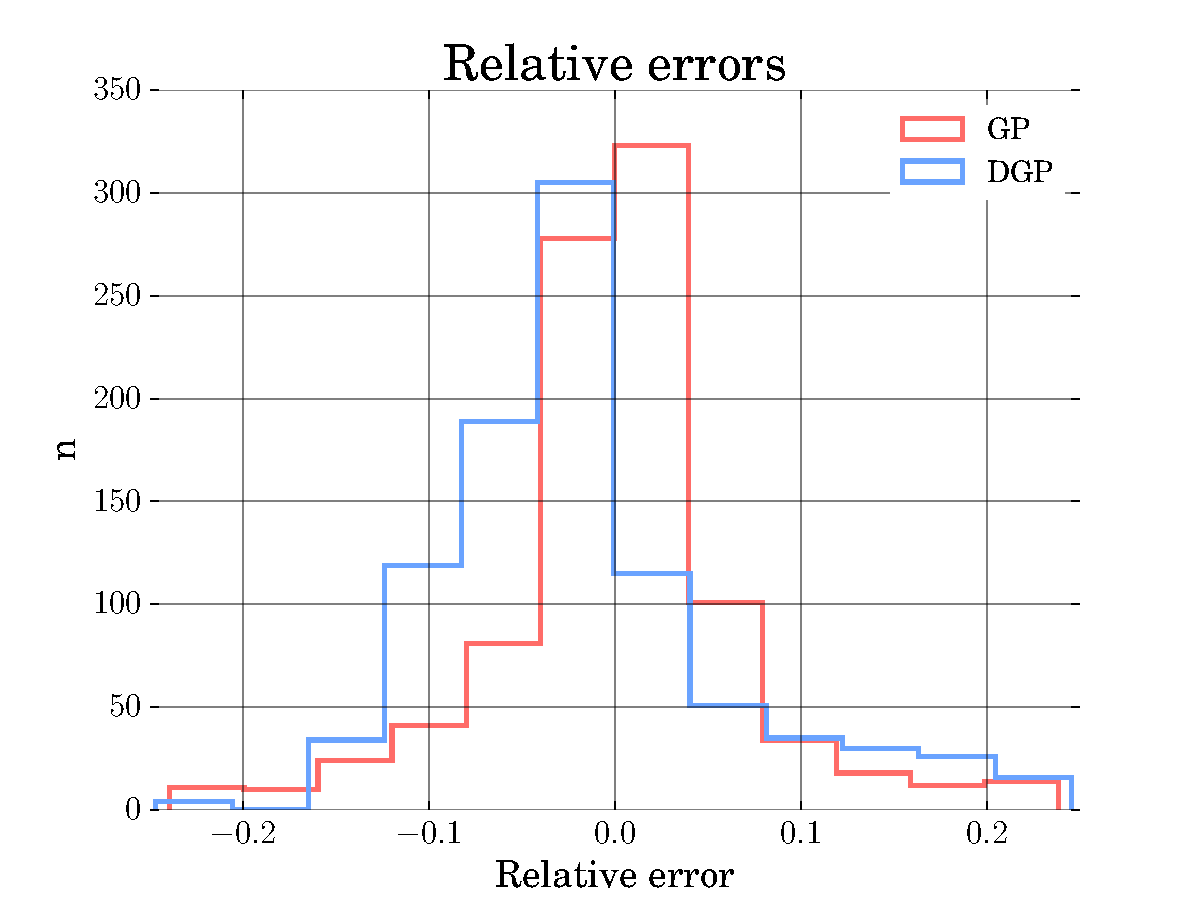
\includegraphics[scale=0.6]{/home/ingrid/Documents/Master/ML/Distributed_GP/testing/DGP_fx.pdf}
\caption{Histograms of the relative errors calculated according to Eq. (\ref{Eq:: rel err}) by Gaussian processes (GP) and Distributed Gaussian processes (DGP) with 2000 points, 1000 training points for the test function in Eq. (\ref{Eq:: test function f(x)}).}
\end{figure}
 
\begin{figure}
\centering
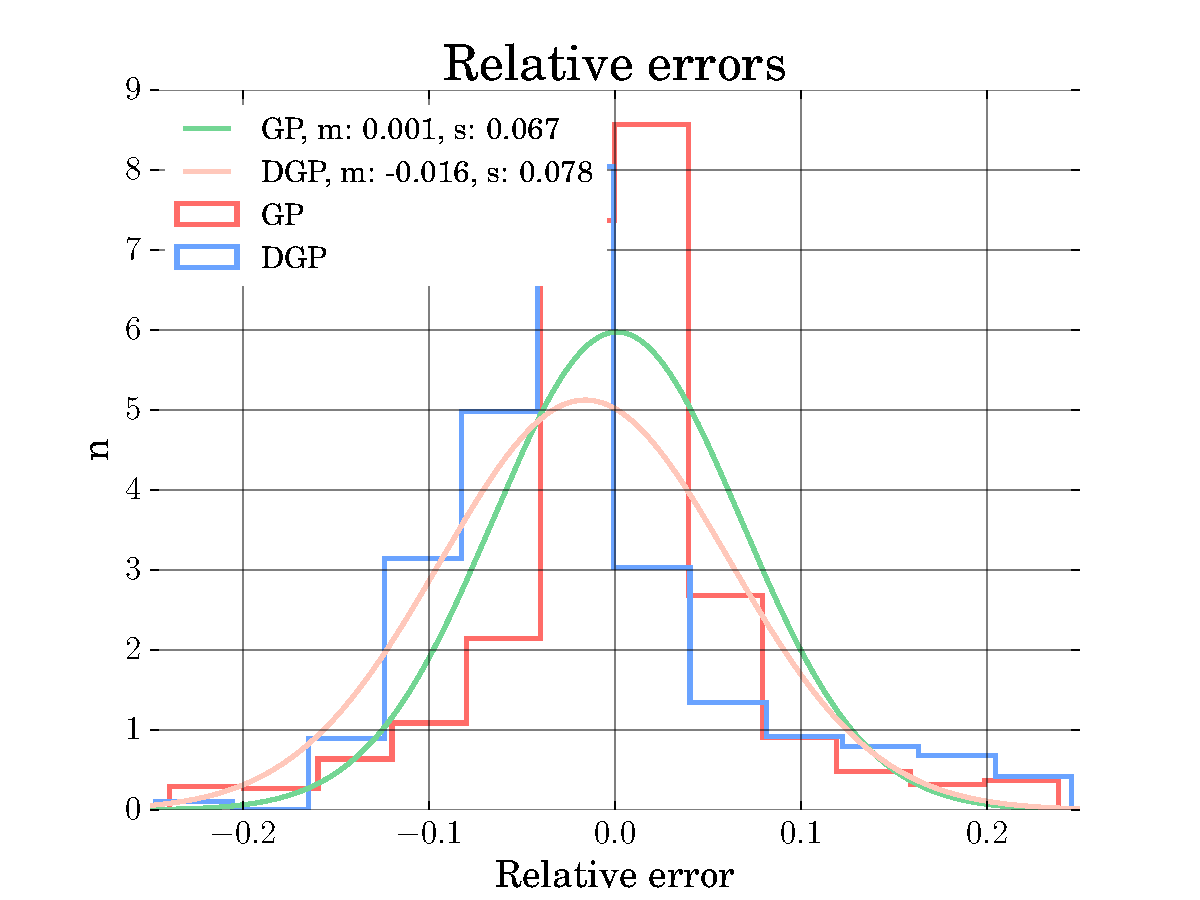
\includegraphics[scale=0.6]{/home/ingrid/Documents/Master/ML/Distributed_GP/testing/DGP_fx_gauss.pdf}
\caption{Normalized histograms of the relative errors calculated according to Eq. (\ref{Eq:: rel err}) by Gaussian processes (GP) and Distributed Gaussian processes (DGP) with 2000 points, 1000 training points for the test function in Eq. (\ref{Eq:: test function f(x)}). Gaussian curves are fitted for each, with mean $m$ and variance $s$.}
\end{figure}


\section*{Improving the kernel}

In trying to use DGP on the actual data set of my thesis, the 20k set, the kernel I was using (RBF+WhiteKernel) proved to be very inefficient. The histogram of errors centered around 1 and the points were spread all over. Changing to what is called $kernel1$ in the scripts, namely $C*RBF$, improved the DGP-approximation considerably. 

Due to the large improvement, I went back and tested the different kernels with regular GP on the 20k data set, using 200 training points. A table of the kernels is found in Tab. ().The results are found in Tab. ().

\begin{table}
\centering
\begin{tabular}{|c|l|}
\hline
Kernel & Specifics\\
\hline
1 & $C(1.0, (1e-2, 1e2)) * RBF(10, (1e-3, 1e3))$\\
\hline
2 & $DotProduct(sigma\_0=1.0, sigma\_0\_bounds=(1e-05, 100.0))$\\
\hline
3 & $ExpSineSquared(length\_scale=10.0, periodicity=1.0,$\\
&$ length\_scale\_bounds=(1e-02, 1000.0), periodicity\_bounds=(1e-02, 1000.0))$\\
\hline
4 & $RBF(936, (1e-2, 1e5))$\\
&$ + WhiteKernel(noise\_level=0.374, noise\_level\_bounds=(1e-10, 1e+2))$\\
\hline
\end{tabular}
\caption{Description of the tested kernels. These are functions in scikit-learn.}
\label{Tab:: kernels list}
\end{table}


\begin{table}
\begin{tabular}{|c|l|l|l|l|}
\hline
Kernel & Fraction & Optimized kernel & $\mu$ & $\sigma$\\
\hline
1 & 0.1665 & $C = 10**2$, $length\_scale=833$ & -0.02154 & 0.19508\\
2 & 0.7988 & $sigma\_0=2.01$ & 0.05088 & 0.29124\\
3 & NA & NA & NA & NA\\
4 & 0.7480 & $length\_scale=2.44e+03$, $ noise\_level=1.78$ & 0.03848 & 0.28073\\
\hline
\end{tabular}
\caption{Tab:: Testing of kernels using 20k data set, and 200 training points. These numbers are for regular Gaussian process approximation. Fraction describes the fraction of points that lie outside the interval [-0.5,0.5], and $\sigma$ and $\mu$ are the mean and variance of the approximated Gaussian distribution.}
\end{table}

The plots of histograms are found in Fig. (\ref{Fig:: GP 20k 200training kernel1})-(\ref{Fig:: GP 20k 200training kernel3}).

\begin{figure}
\centering
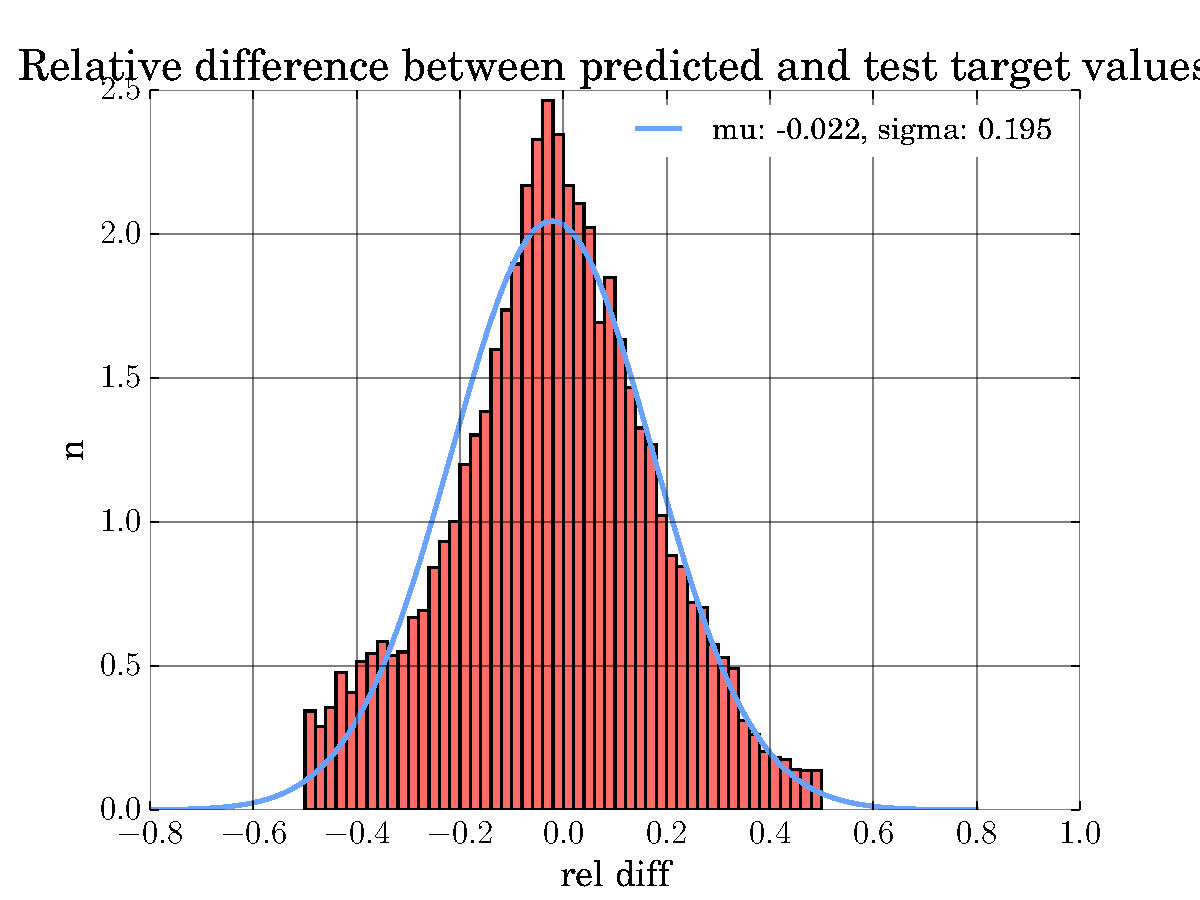
\includegraphics[scale=0.5]{/home/ingrid/Documents/Master/ML/Abel_lin_log_20000/kernels/kernel1.pdf}
\caption{Histogram of relative errors calculated according to Eq. (\ref{Eq:: rel err}), using GP on 20k data set, with 200 training points. The kernel used was $kernel1$, according to Tab. \ref{Tab:: kernels list}. $16.65 \%$ of the points are not shown in the histogram, as these lie outside the interval $[-0.5, 0.5]$.}
\label{Fig:: GP 20k 200training kernel1}
\end{figure}

\begin{figure}
\centering
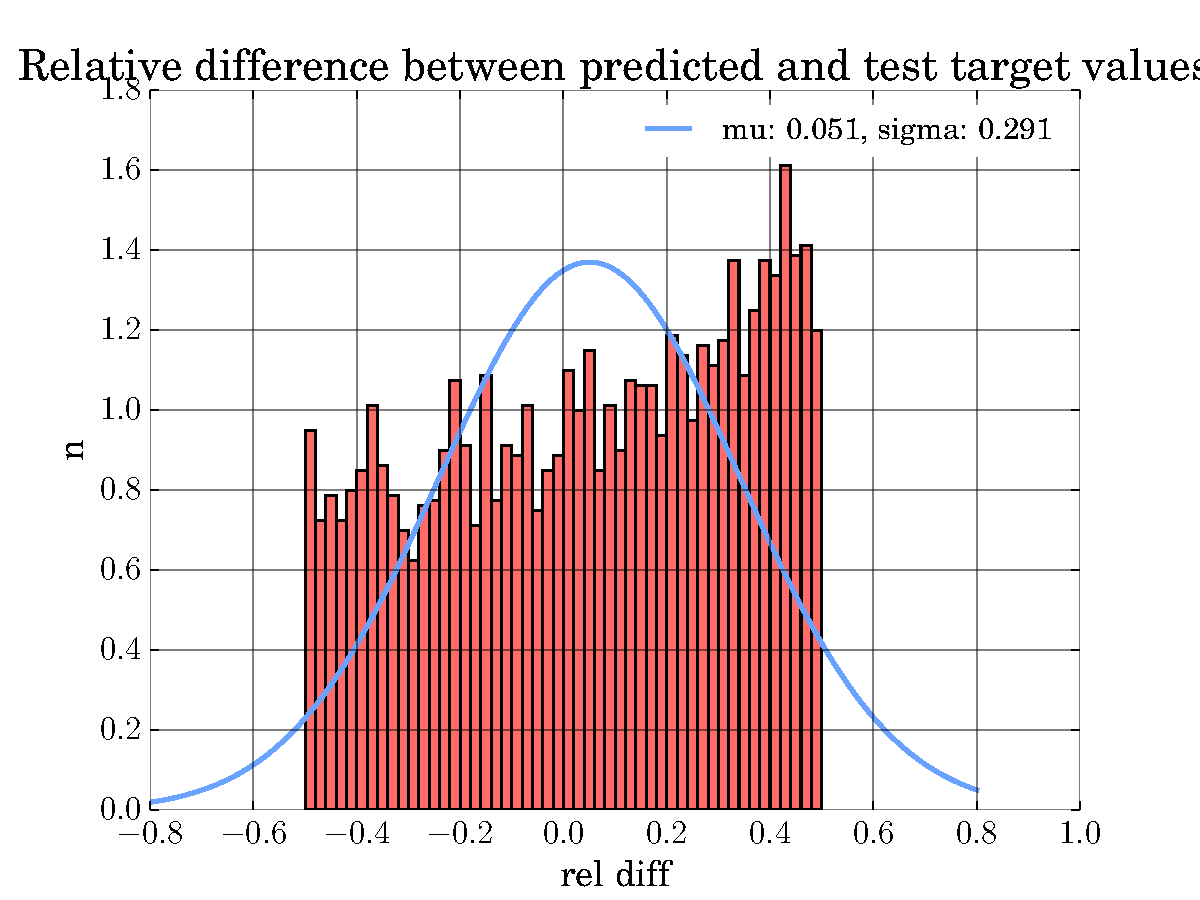
\includegraphics[scale=0.5]{/home/ingrid/Documents/Master/ML/Abel_lin_log_20000/kernels/kernel2}
\caption{Histogram of relative errors calculated according to Eq. (\ref{Eq:: rel err}), using GP on 20k data set, with 200 training points. The kernel used was $kernel2$, according to Tab. \ref{Tab:: kernels list}. $79.88 \%$ of the points are not shown in the histogram, as these lie outside the interval $[-0.5, 0.5]$.}
\label{Fig:: GP 20k 200training kernel2}
\end{figure}

\begin{figure}
\centering
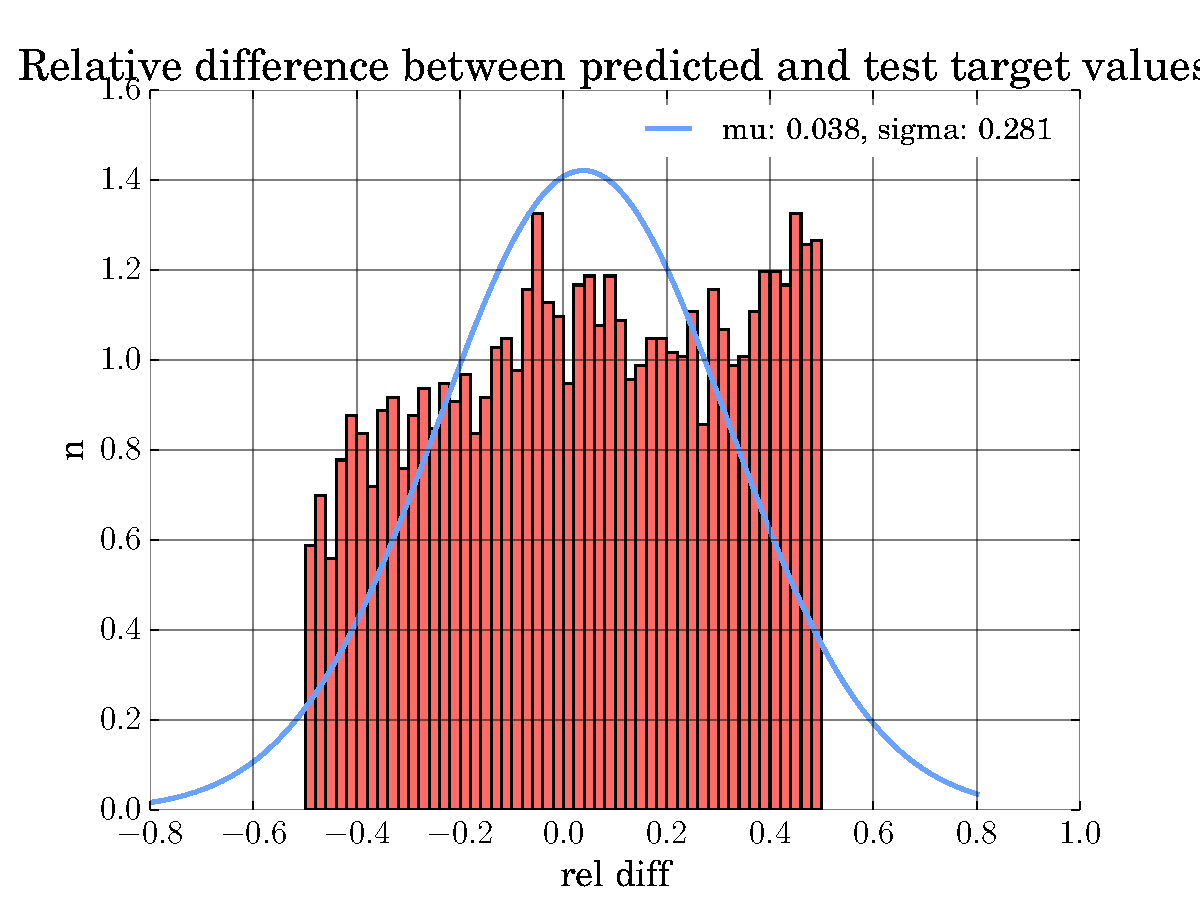
\includegraphics[scale=0.5]{/home/ingrid/Documents/Master/ML/Abel_lin_log_20000/kernels/kernel4}
\caption{Histogram of relative errors calculated according to Eq. (\ref{Eq:: rel err}), using GP on 20k data set, with 200 training points. The kernel used was $kernel4$, according to Tab. \ref{Tab:: kernels list}. $74.80 \%$ of the points are not shown in the histogram, as these lie outside the interval $[-0.5, 0.5]$.}
\label{Fig:: GP 20k 200training kernel3}
\end{figure}


\subsection{Distributed GP}
 
For the new kernel, $kernel1$, DGP were tested on the 20k data set. For 200 training points the approximation is quite bad, while for 2000 the approximation is almost as good as GP for 200 training points. Plots are shown in Fig. ().
 
 \subsubsection{8 experts}
 
%\begin{figure}[H]
%\centering
%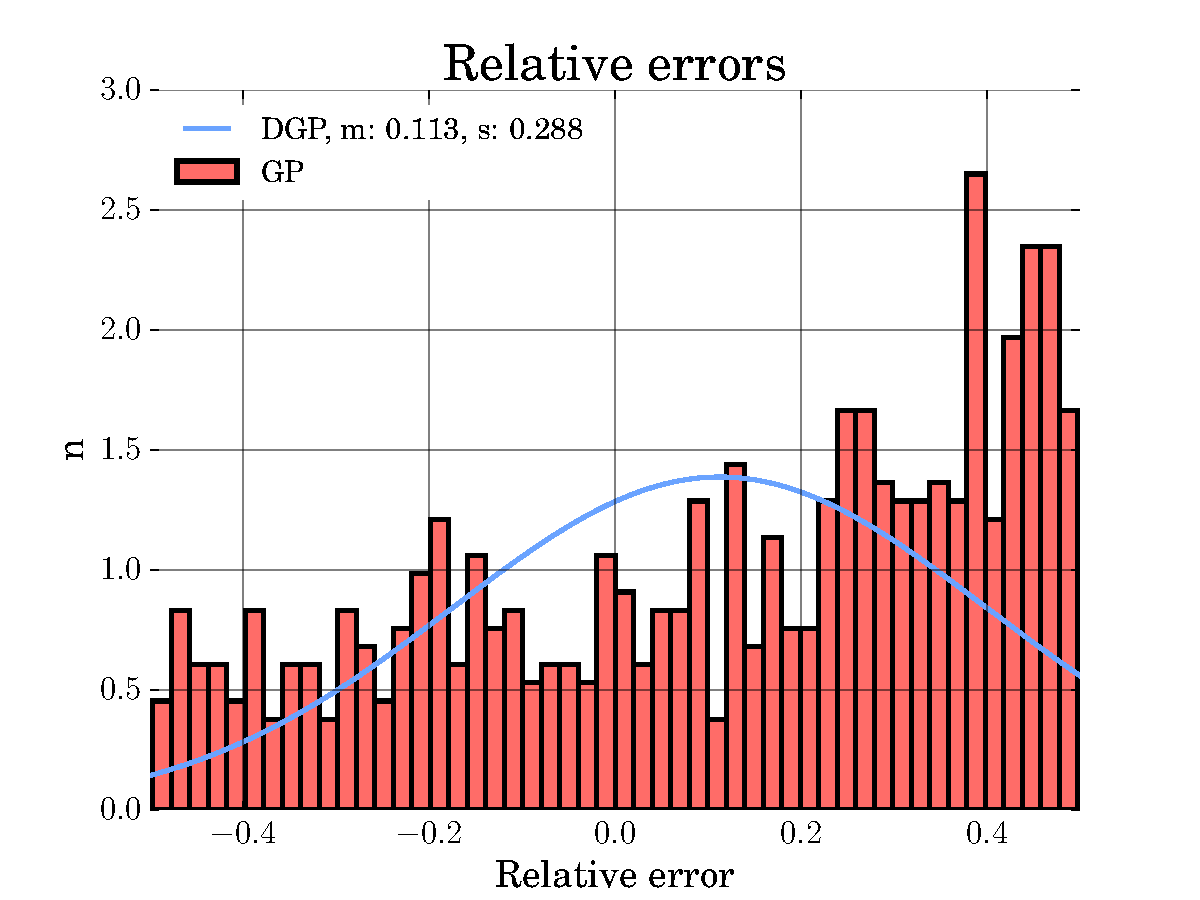
\includegraphics[scale=0.5]{/home/ingrid/Documents/Master/ML/Distributed_GP/Abel_20k_8experts/DGP_pears_001_gauss.pdf}
%\caption{Histogram of relative errors calculated according to Eq. (\ref{Eq:: rel err}), using DGP with 8 experts on 20k data set, with 200 training points. The kernel used was $kernel1$, according to Tab. \ref{Tab:: kernels list}. $96.66 \%$ of the points are not shown in the histogram, as these lie outside the interval $[-0.5, 0.5]$.}
%\label{Fig:: DGP 20k 200training kernel1}
%\end{figure}
 
%\begin{figure}[H]
%\centering
%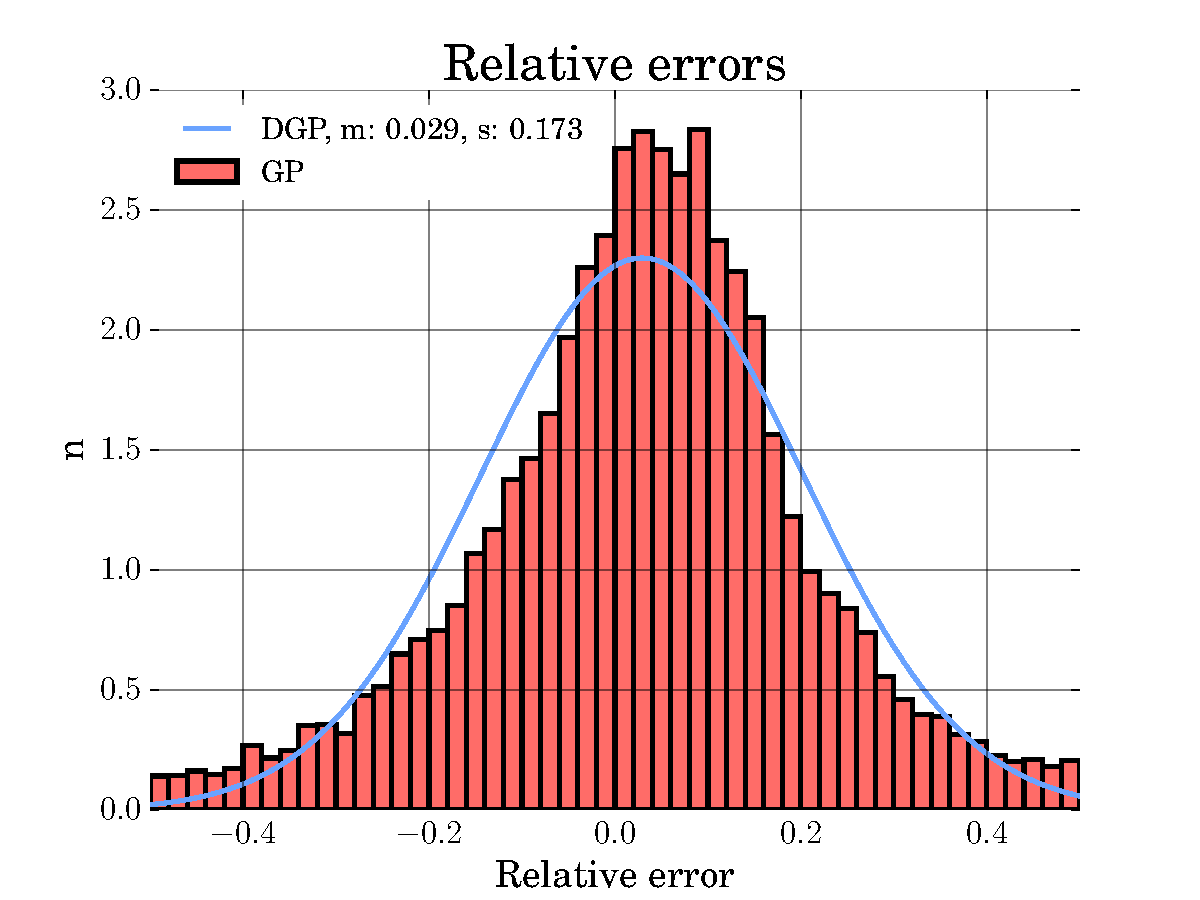
\includegraphics[scale=0.5]{/home/ingrid/Documents/Master/ML/Distributed_GP/Abel_20k_8experts/DGP_pears_01_gauss.pdf}
%\caption{Histogram of relative errors calculated according to Eq. (\ref{Eq:: rel err}), using DGP with 8 experts on 20k data set, with 2000 training points. The kernel used was $kernel1$, according to Tab. \ref{Tab:: kernels list}. $8.13 \%$ of the points are not shown in the histogram, as these lie outside the interval $[-0.5, 0.5]$.}
%\label{Fig:: DGP 20k 2000training kernel1}
%\end{figure}
 
%\begin{figure}[H]
%\centering
%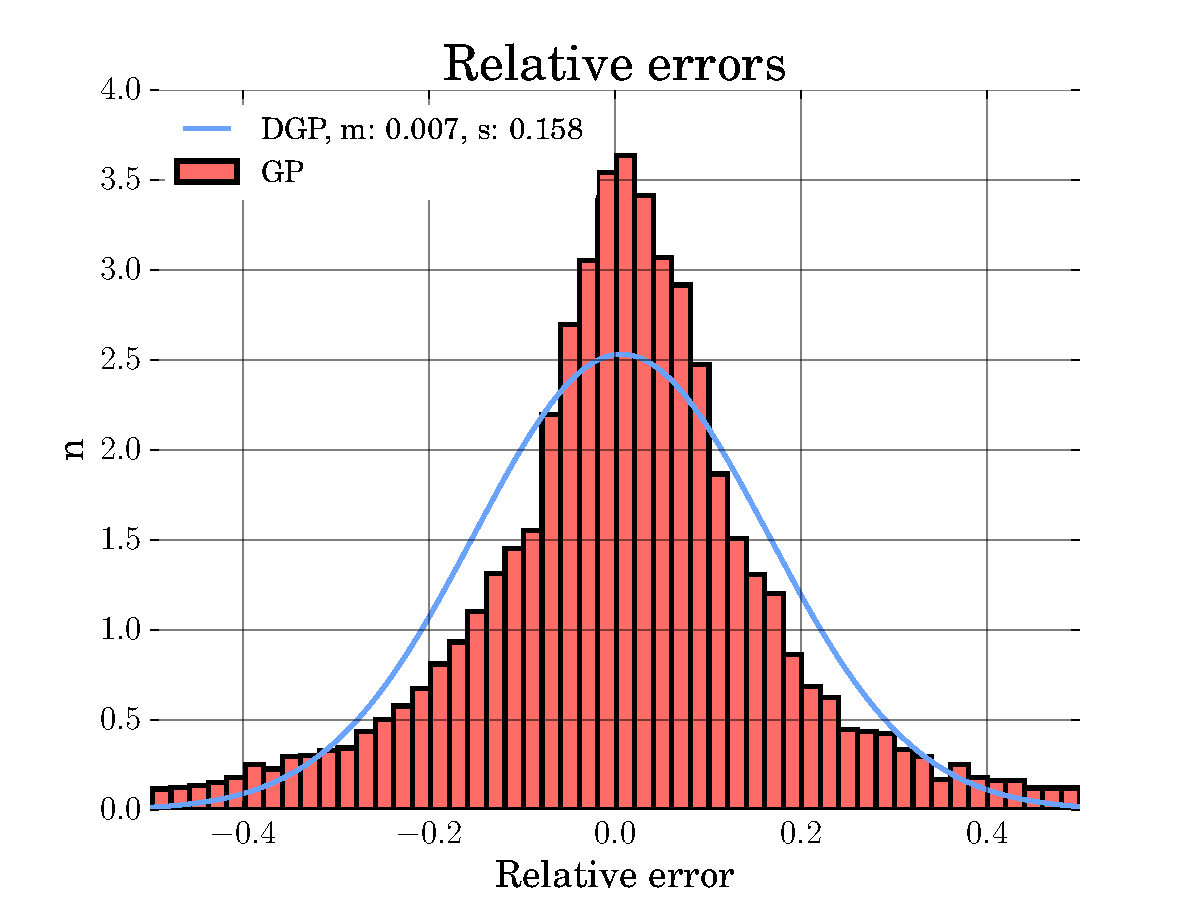
\includegraphics[scale=0.5]{/home/ingrid/Documents/Master/ML/Distributed_GP/Abel_20k_8experts/DGP_pears_05_gauss.pdf}
%\caption{Histogram of relative errors calculated according to Eq. (\ref{Eq:: rel err}), using DGP with 8 experts on 20k data set, with 10000 training points. The kernel used was $kernel1$, according to Tab. \ref{Tab:: kernels list}. $5.96 \%$ of the points are not shown in the histogram, as these lie outside the interval $[-0.5, 0.5]$.}
%\label{Fig:: DGP 20k 10000training kernel1}
%\end{figure} 

To do a further analysis of the 10k training set, I set the limits down to $[-0.25, 0.25]$. This meant excluding $17,5 \%$ of the test points, but gave a very nice approximation with $\sigma = 0.106$, which is very close to the desired number. This plot can be seen in Fig. (\ref{Fig:: DGP 20k 10000training kernel1 small lim}). There is, however, still a small shift in the $\mu$-value, at $\mu = 0.008$, which would ideally be at $\mu= 0$.

\begin{figure}
\centering
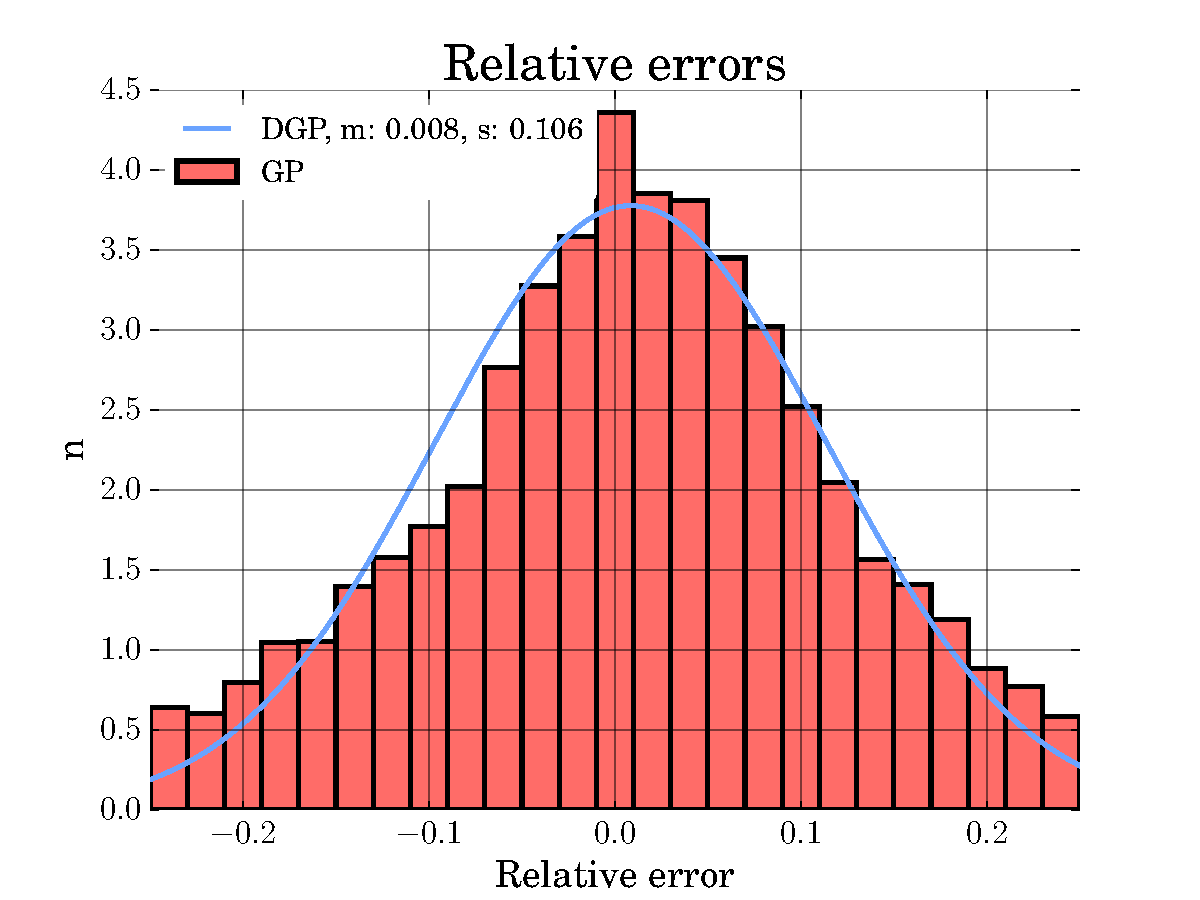
\includegraphics[scale=0.5]{/home/ingrid/Documents/Master/ML/Distributed_GP/Abel_20k_8experts/useless_plots/DGP_pears_05_gauss_smallim.pdf}
\caption{Histogram of relative errors calculated according to Eq. (\ref{Eq:: rel err}), using DGP with 8 experts on 20k data set, with 10000 training points. The kernel used was $kernel1$, according to Tab. \ref{Tab:: kernels list}. $17.51 \%$ of the points are not shown in the histogram, as these lie outside the interval $[-0.25, 0.25]$.}
\label{Fig:: DGP 20k 10000training kernel1 small lim}
\end{figure}
 
Visualizing the experts' calculations is found in Fig. ().

\begin{figure}
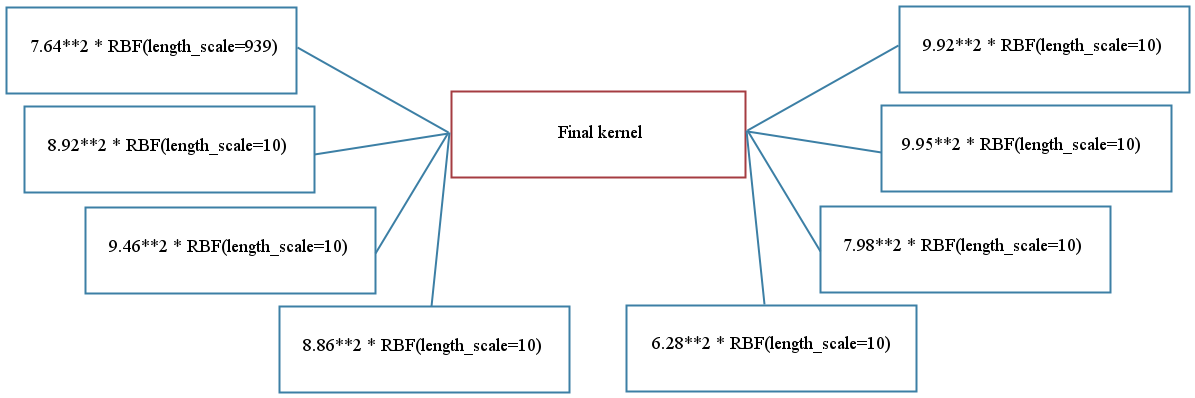
\includegraphics[scale=0.4]{/home/ingrid/Documents/Master/ML/Distributed_GP/Abel_20k_8experts/DGP_experts_visual_8exp_001.png}
\caption{Calculations of individual experts using 200 training points.}
\label{Fig:: visualizing 8 experts 0.001}
\end{figure}
 
 
\subsubsection{4 experts} 
 
%\begin{figure}[H]
%\centering
%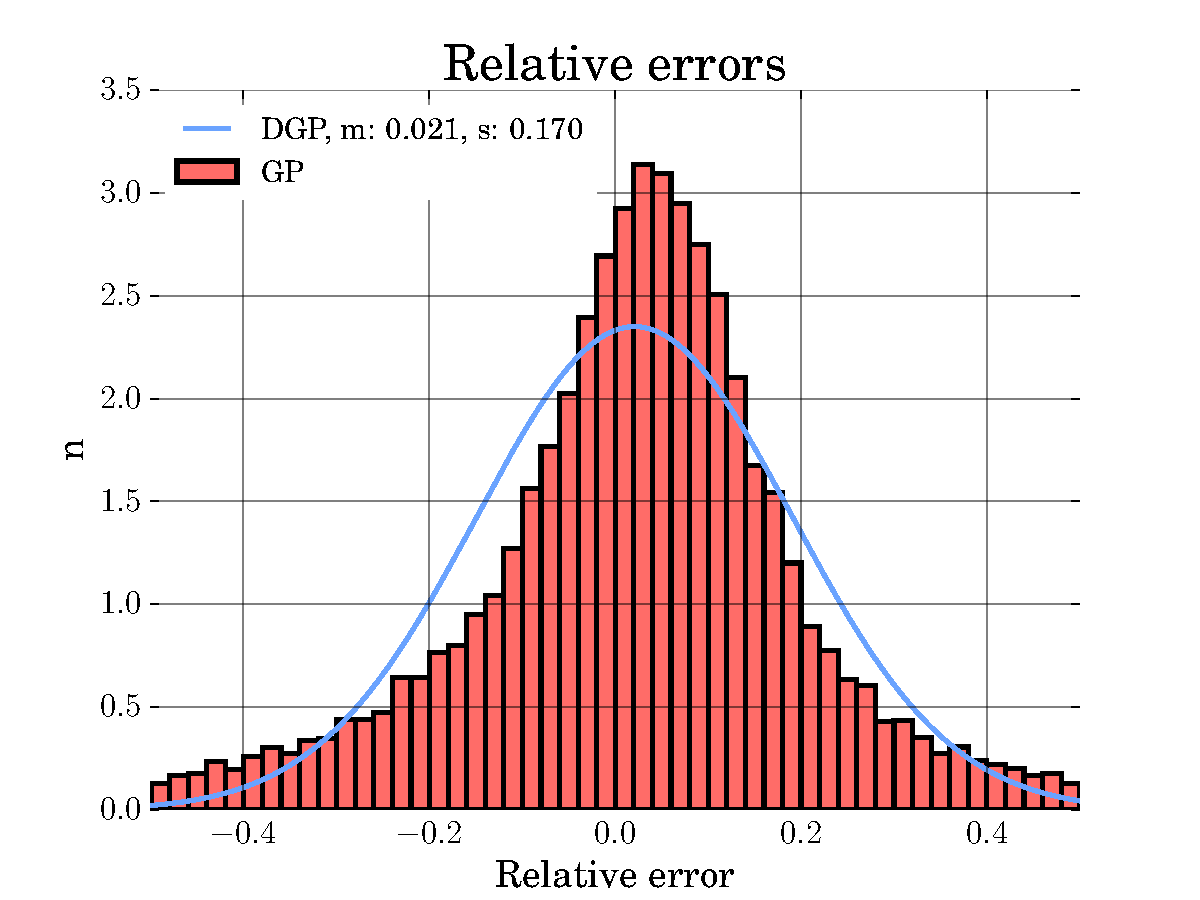
\includegraphics[scale=0.5]{/home/ingrid/Documents/Master/ML/Distributed_GP/Abel_20k_4experts/DGP_pears_gauss_01.pdf}
%\caption{Histogram of relative errors calculated according to Eq. (\ref{Eq:: rel err}), using DGP with 4 experts on 20k data set, with 2000 training points. The kernel used was $kernel1$, according to Tab. \ref{Tab:: kernels list}. $8.78 \%$ of the points are not shown in the histogram, as these lie outside the interval $[-0.5, 0.5]$.}
%\label{Fig:: DGP 20k 2000training kernel1}
%\end{figure} 
 
 
\begin{figure}
\centering
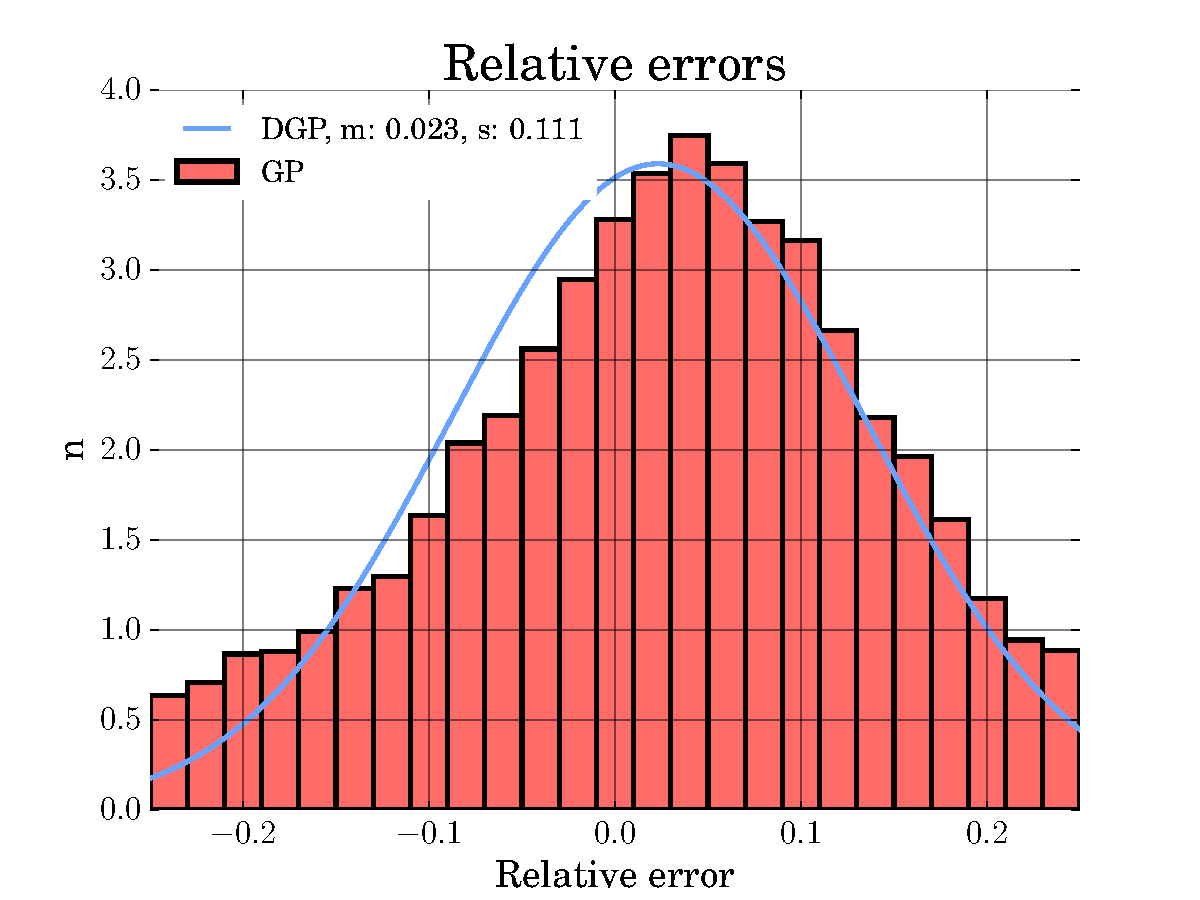
\includegraphics[scale=0.5]{/home/ingrid/Documents/Master/ML/Distributed_GP/Abel_20k_4experts/useless_plots/DGP_pears_01_gauss_smallim.pdf}
\caption{Histogram of relative errors calculated according to Eq. (\ref{Eq:: rel err}), using DGP with 4 experts on 20k data set, with 2000 training points. The kernel used was $kernel1$, according to Tab. \ref{Tab:: kernels list}. $22.19 \%$ of the points are not shown in the histogram, as these lie outside the interval $[-0.25, 0.25]$.}
\label{Fig:: DGP 20k 2000training kernel1}
\end{figure}  
 
 
%\begin{figure}[H]
%\centering
%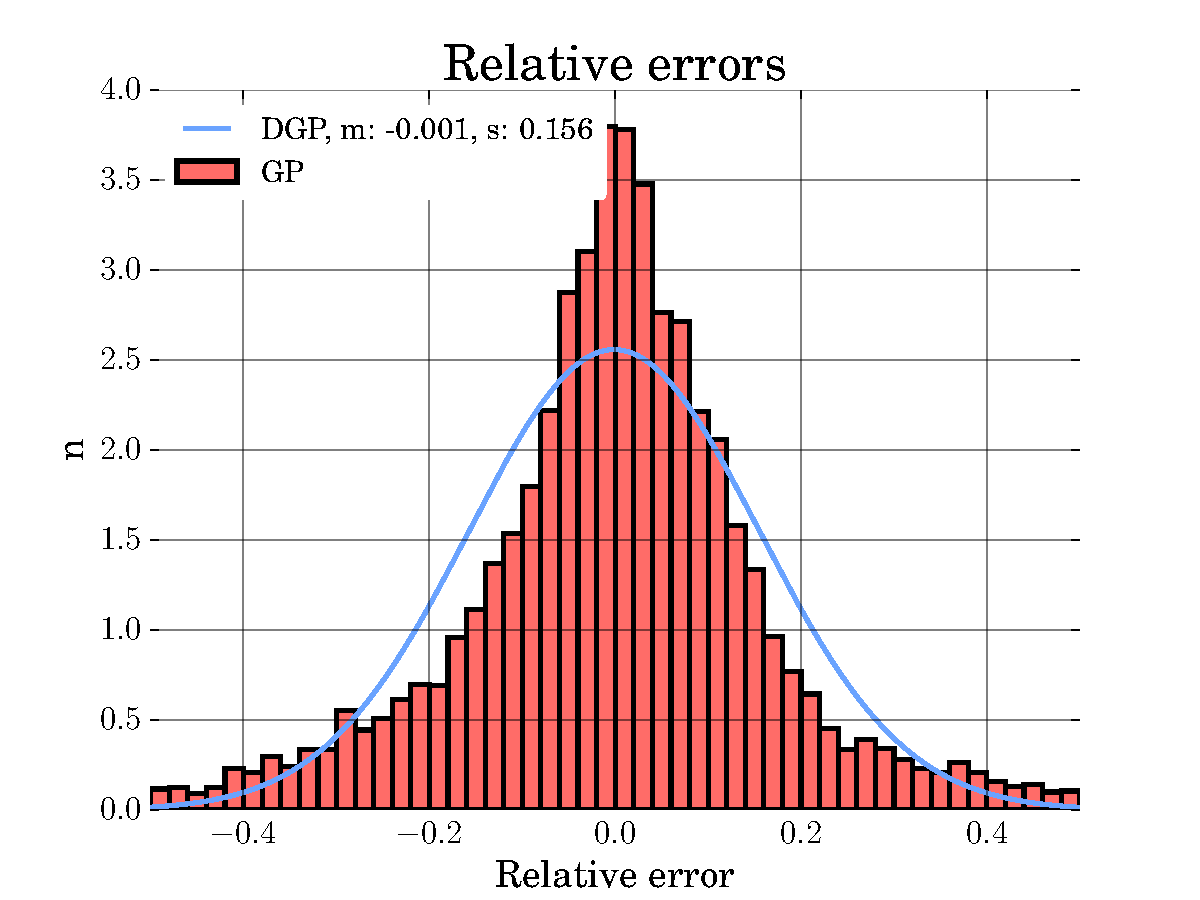
\includegraphics[scale=0.5]{/home/ingrid/Documents/Master/ML/Distributed_GP/Abel_20k_4experts/DGP_pears_gauss_05.pdf}
%\caption{Histogram of relative errors calculated according to Eq. (\ref{Eq:: rel err}), using DGP with 4 experts on 20k data set, with 10000 training points. The kernel used was $kernel1$, according to Tab. \ref{Tab:: kernels list}. $5.81 \%$ of the points are not shown in the histogram, as these lie outside the interval $[-0.5, 0.5]$.}
%\label{Fig:: DGP 20k 10000training kernel1}
%\end{figure} 
 
 
\begin{figure}
\centering
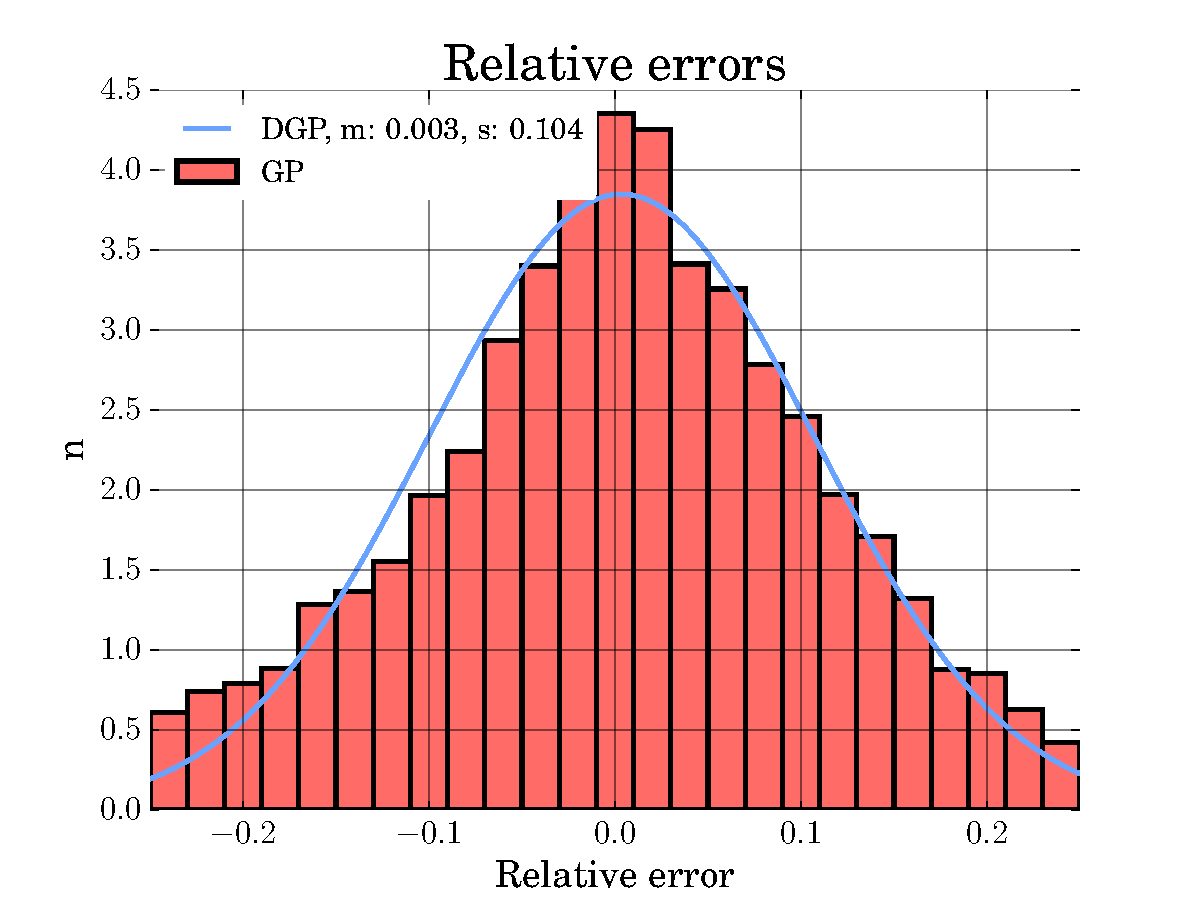
\includegraphics[scale=0.5]{/home/ingrid/Documents/Master/ML/Distributed_GP/Abel_20k_4experts/useless_plots/DGP_pears_gauss_05_smallims.pdf}
\caption{Histogram of relative errors calculated according to Eq. (\ref{Eq:: rel err}), using DGP with 4 experts on 20k data set, with 10000 training points. The kernel used was $kernel1$, according to Tab. \ref{Tab:: kernels list}. $17.35 \%$ of the points are not shown in the histogram, as these lie outside the interval $[-0.25, 0.25]$.}
\label{Fig:: DGP 20k 10000training kernel1}
\end{figure}
 

 
Using 4 experts gives a better results, but takes much longer to calculate, as the matrices are much larger. The improvement in quality is not large enough to compensate for the calculation time. 
 
\begin{table}
\centering
\begin{tabular}{|c|l|l|l|l|}
\hline
Number of experts & Training size & $\mu$ & $\sigma$ & Fraction\\
\hline
4 & 2000 & 0.023 & 0.111 & $22.19 \%$\\
4 & 10 000 & 0.003 & 0.104 & $17.35 \%$\\
8 & 200 & 0.113* & 0.288*  & $96.66 \%$* \\
8 & 2000 & 0.024 & 0.115 & $22.54 \%$\\
8 & 10 000 & 0.008 & 0.106 & $17.51 \%$\\
\hline
\end{tabular}
\caption{DGP on 20k data set for the interval $[-0.25, 0.25]$. For values marked by *, the interval $[-0.5,0.5]$ has been used.}
\label{Tab:: DGP comparison of mu sigma for 4 8 exp}
\end{table}

An analysis of the CPU time can be found in Tab. . The computations were made on a laptop with 4 cores (SJEKK DETTE).

\begin{table}
\centering
\begin{tabular}{|c|l|l|l|}
\hline
 & 200 training points & 2000 training points & 10 000 training points\\
 \hline
8 experts & 0m35.209s & 0m55.074s & 9m3.439s\\
4 experts & 0m17.884s & 1m10.176s & 25m1.591s\\
\hline
\end{tabular}
\caption{Calculation time for a laptop to perform the non-parallelized DGP on the 20k data set. The time was calculated by using $time$ before the $python$ statement.}
\end{table}
 
\section{Parallelizing the algorithm} 
 
 
The algorithm should be parallelized by dividing the number of experts by the number of cores available. These should both be multiples of 4, for simplicity.
\begin{align}
N = \frac{N_{experts}}{N_{cores}}.
\end{align} 
Each core should do calculations for $N$ experts, and the core with rank 0 should sum up numbers and find $\mu_{rbcm}$ and $\sigma_{rbcm}$. The section that seems the most advantageous to parallelize is the first $for$-loop block in Algorithm (\ref{Alg:: DGP}). Then each core should be assigned a number of experts, for which it does the time- and memory consuming DGP fit.

\subsection{Benchmark for parallelization}

In order to test the parallelization algorithm a benchmark program was made, usng the same routine. This routine should divide the job between experts, again distributed amongst the nodes. Assume there are $N$ experts. Each expert $j$ should perform the same calulation, where input vectors should be $\textbf{x}_j \in \mathbb{R}^m$ and $\textbf{x}_* \in \mathbb{R}^{n}$. Output vectors for each expert should be $\textbf{y}_{i*} \in \mathbb{R}^n$, and the final output should be some linear combination of these $\textbf{y}_{tot *} = \textbf{h}^T \textbf{y}_*$. A somple example is given by
\begin{align}
\text{For each expert j: } & f_j = f(\textbf{x}_j) = \sum_{k=1}^m x_{j k},\\
& \textbf{g}_j = g (\textbf{y}_*, f(\textbf{x}_j)) = f_j \cdot \textbf{y}_*,\\
\text{Summing node: } & \textbf{y}_{tot *} = G(\textbf{y}_*) = \frac{1}{N} \sum_{j=1}^N \textbf{g}_j.
\end{align}

An important challenge here is to make the routine \textbf{load balancing}. Since the experts are divided between cores, it is imperative that a clever distribution is found. Giving the rest to a single core, for example, is a very inefficient solution.


\subsection{GridSearchCV from scikitlearn}

After trying to parallelize with MPI4PY and running into some complications, I've decided to look at how GridSearch (a scikitlearn module) is parallelized. 

\subsection{Results: 4 experts}

Since the previous sections concluded with the superiority of $kernel6$, this is the kernel that has been used for further testing of the module. Computational time for the parallelized DGP module can be found in Tab. (\ref{Tab:: Calc time for parallelized}).

\begin{table}
\centering
\begin{tabular}{|c|l|l|l|}
\hline
 & 200 training points & 2000 training points & 10 000 training points\\
 \hline
8 experts & 0m17.056s & 0m25.552s & 4m30.017s \\
4 experts & 0m9.184s & 0m28.395s & 9m37.533s\\
\hline
\end{tabular}
\caption{Calculation time for a laptop to perform the parallelized DGP on the 20k data set. The time was calculated by using $time$ before the $python$ statement.}
\label{Tab:: Calc time for parallelized}
\end{table}

The fraction of points outside the intervals $[-0.5, 0.5]$ and $[-0.25, 0.25]$, along with the Gaussian approximation parameters can be found in Tab. (\ref{Tab:: DGP parallel 20k 4 experts comparison of training fractions k6})-().

\begin{table}
\centering
\begin{tabular}{ccccccc}
\toprule
Training fraction &  \multicolumn{3}{c}{$[-0.5, 0.5]$} & \multicolumn{3}{c}{$[-0.25,0.25]$}\\
\midrule
{}  & $\mu$ & $\sigma^2$ & $n/N$ & $\mu$ & $\sigma^2$ & $n/N$\\
0.01 & 0.014 & 0.215 & 0.2107 & 0.011 & 0.127 & 0.4205\\
0.1 & 0.028 & 0.183 & 0.0931 & 0.025 & 0.117 & 0.2566\\
0.5 & 0.006 & 0.161 & 0.0575 & 0.007 & 0.108 & 0.1823\\
\bottomrule
\end{tabular}
\caption{Gaussian fit parameters for the parallelized 20 000 point Distributed Gaussian Process approximations, using kernel 6 ($k = C_1 \exp (-x^2/\ell^2) + C_2$, where $C_1, C_2$ are constants) and 4 experts. The parameter $n/N$ is the fraction of test points that lies outside the given interval.}
\label{Tab:: DGP parallel 20k 4 experts comparison of training fractions k6}
\end{table}

\begin{table}
\centering
\begin{tabular}{ccccccc}
\toprule
Training fraction &  \multicolumn{3}{c}{$[-0.5, 0.5]$} & \multicolumn{3}{c}{$[-0.25,0.25]$}\\
\midrule
{}  & $\mu$ & $\sigma^2$ & $n/N$ & $\mu$ & $\sigma^2$ & $n/N$\\
0.01 & -0.049 & 0.216 & 0.5255 & -0.010 & 0.131 & 0.6594\\
0.1 & 0.037 & 0.176 & 0.0825 & 0.025 & 0.113 & 0.2393\\
0.5 & 0.013 & 0.161 & 0.0586 & 0.015 & 0.107 & 0.1806\\
\bottomrule
\end{tabular}
\caption{Gaussian fit parameters for the parallelized 20 000 point Distributed Gaussian Process approximations, using kernel 6 ($k = C_1 \exp (-x^2/\ell^2) + C_2$, where $C_1, C_2$ are constants) and 4 experts. The parameter $n/N$ is the fraction of test points that lies outside the given interval.}
\label{Tab:: DGP parallel 20k 8 experts comparison of training fractions k6}
\end{table}

Running DGP parallelized with 8 experts on a laptop with 4 nodes gives the errors shown in Fig. (\ref{Fig:: DGP parallel 8 exp 4 nodes kernel 6 error histogram}).

\begin{figure}
\centering
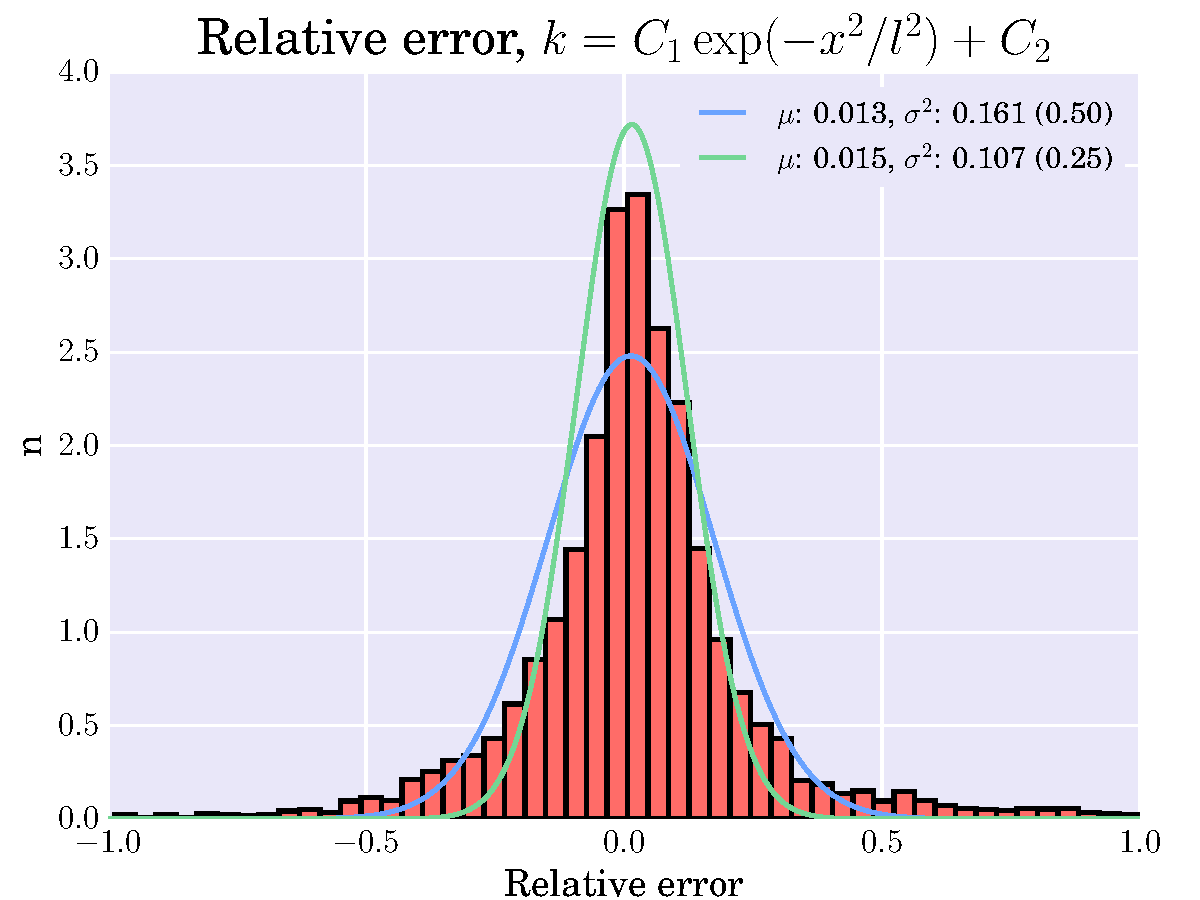
\includegraphics[scale=0.6]{/home/ingrid/Documents/Master/ML/Distributed_GP/Abel_20k_8experts_parallel/plots/errors_k6_05.pdf}
\caption{ Histogram of relative errors calculated according to Eq. (\ref{Eq:: rel err}), using parallelized DGP with 8 experts on 20k data set, with 10000 training points. The kernel used was $kernel6$, according to Tab. (\ref{Tab:: kernels list}). The fraction of points outside of the interval $[-1.0,1.0]$ is $0.012$.}
\label{Fig:: DGP parallel 8 exp 4 nodes kernel 6 error histogram}
\end{figure}




\bibliographystyle{plain}
\bibliography{DGP_kapittel}

\end{document}

